\documentclass{beamer}
\usepackage[utf8]{inputenc}
\usepackage{tikz}
\usepackage[dvipsnames,svgnames,table,hyperref]{xcolor}
\usetikzlibrary{calc, arrows}
\usetikzlibrary{shapes.multipart} %for the stack
\usepackage{listings} 
\usepackage{mathtools}
\usepackage{amsthm}
\usepackage{kbordermatrix} %for the representations
\pgfdeclarelayer{background} %tiks animation stuff
\pgfsetlayers{background,main}
\usetheme{metropolis}           % Use metropolis theme
\title{Graph Theory}
\date{\today}
\author{Dadams, TEC, Nick, Tom}
\institute{Graph This!}

\begin{document}
  \maketitle
  \section{Warning: Graphic Content Ahead}
  \begin{frame}{What is a Graph}
\begin{center}
    This is a graph
\end{center}
    \tikzset{vertex/.style={draw=red!40!white, black=red, fill=red!10!white, shape=circle, inner sep=0.5pt, minimum size=16pt}}
    \begin{tikzpicture}[
            g1v/.style={vertex,draw=red!40!white, black=red, fill=red!10!white},
            g2v/.style={vertex,draw=blue!40!white, black=blue, fill=blue!10!white},
            g3v/.style={vertex,draw=green!40!white, black=green, fill=green!10!white},
            scale=2
        ]
        \node[g1v] (0) at (0,0.75) {0};

        \node[g1v] (1) at (1.5,1.5) {1};
        \node[g3v] (2) at (1.5,0) {2};

        \node[g2v] (3) at (3,1.5) {3};
        \node[g3v] (4) at (3,0) {4};

        \node[g1v] (5) at (4.5,1.5) {5};

        \draw[] (0) -- node[above] {7} (1);
        \draw[] (1) -- node[left] {4} (2);
        \draw[->,] (1) -- (3);
        \draw[] (1) -- (4);
        \draw[->,] (2) -- (0);
        \draw[] (2) -- node[below] {8} (4);
        \draw[] (3) -- (5);
    \end{tikzpicture}
    
  \end{frame}
  \begin{frame}{What is not a Graph}
  
    \begin{columns}
    
    \column{0.6\textwidth}
    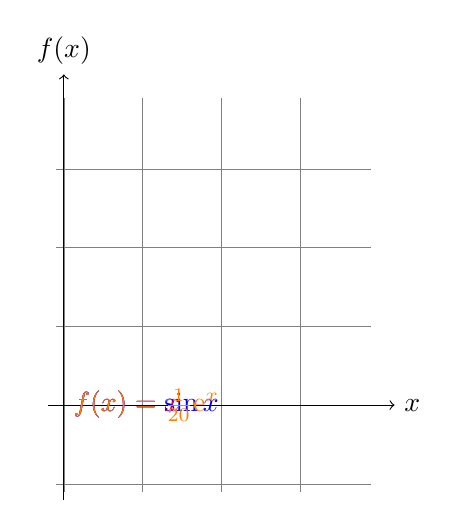
\begin{tikzpicture}[domain=0:4]
    \draw[very thin,color=gray] (-0.1,-1.1) grid (3.9,3.9);
    \draw[->] (-0.2,0) -- (4.2,0) node[right] {$x$};
    \draw[->] (0,-1.2) -- (0,4.2) node[above] {$f(x)$};
    \draw[color=red] plot[id=x] function{x} 
        node[right] {$f(x) =x$};
    \draw[color=blue] plot[id=sin] function{sin(x)} 
        node[right] {$f(x) = \sin x$};
    \draw[color=orange] plot[id=exp] function{0.05*exp(x)} 
        node[right] {$f(x) = \frac{1}{20} \mathrm e^x$};
   \end{tikzpicture}
    
    \column{0.4\textwidth}
    \begin{itemize}
        \item This is a \textbf{PLOT}
        \item Don't let anyone else tell you otherwise
    \end{itemize}
    \end{columns}
      
  \end{frame}
  \begin{frame}{If your a mathematician}
      \begin{definition}
        a \alert{simple graph} denoted \(G(V,E)\) consists of a non-empty set \(V\) of \alert{vertices} and a set \(E\) of \alert{edges} such that each edge \(e \in E\) is associated with an un-ordered pair of distinct vertices, called its endpoints
      \end{definition}
  \end{frame}
  \begin{frame}{For the rest of us}
  \tikzset{vertex/.style={draw=red!40!white, black=red, fill=red!10!white, shape=circle, inner sep=0.5pt, minimum size=16pt}}
        \begin{tikzpicture}[
            g1v/.style={vertex,draw=red!40!white, black=red, fill=white!10!white},
            g2v/.style={vertex,draw=blue!40!white, black=blue, fill=white!10!white},
            g3v/.style={vertex,draw=green!40!white, black=green, fill=white!10!white},
            scale=2
        ]
        \node[g1v] (0) at (0,0.75) {0};

        \node[g1v] (1) at (1.5,1.5) {1};
        \node[g3v] (2) at (1.5,0) {2};

        \node[g2v] (3) at (3,1.5) {3};
        \node[g3v] (4) at (3,0) {4};

        \node[g1v] (5) at (4.5,1.5) {5};

        \draw[] (0) --  (1);
        \draw[] (1) --  (2);
        \draw[] (1) -- (3);
        \draw[] (1) -- (4);
        \draw[] (2) -- (0);
        \draw[] (2) -- (4);
        \draw[] (3) -- (5);
    \end{tikzpicture}
    \begin{center}
        vertices and edges
    \end{center}
  \end{frame}
    \begin{frame}{For the rest of us}
    \tikzset{vertex/.style={draw=red!40!white, black=red, fill=red!10!white, shape=circle, inner sep=0.5pt, minimum size=16pt}}
        \begin{tikzpicture}[
            g1v/.style={vertex,draw=red!40!white, black=red, fill=white!10!white},
            g2v/.style={vertex,draw=blue!40!white, black=blue, fill=white!10!white},
            g3v/.style={vertex,draw=green!40!white, black=green, fill=white!10!white},
            g4v/.style={vertex,draw=green!40!white, black=green, fill=red!10!white},
            scale=2
        ]
        \node[g1v] (0) at (0,0.75) {0};

        \node[g1v] (1) at (1.5,1.5) {1};
        \node[g4v] (2) at (1.5,0) {2};

        \node[g2v] (3) at (3,1.5) {3};
        \node[g3v] (4) at (3,0) {4};

        \node[g1v] (5) at (4.5,1.5) {5};

        \draw[] (0) --  (1);
        \draw[] (1) --  (2);
        \draw[] (1) -- (3);
        \draw[] (1) -- (4);
        \draw[] (2) -- (0);
        \draw[] (2) -- (4);
        \draw[thick] (3) -- (5);
    \end{tikzpicture}
    \begin{center}
        vertices
    \end{center}
  \end{frame}
      \begin{frame}{For the rest of us}
      \tikzset{vertex/.style={draw=red!40!white, black=red, fill=red!10!white, shape=circle, inner sep=0.5pt, minimum size=16pt}}
        \begin{tikzpicture}[
            g1v/.style={vertex,draw=red!40!white, black=red, fill=white!10!white},
            g2v/.style={vertex,draw=blue!40!white, black=blue, fill=white!10!white},
            g3v/.style={vertex,draw=green!40!white, black=green, fill=white!10!white},
            scale=2
        ]
        \node[g1v] (0) at (0,0.75) {0};

        \node[g1v] (1) at (1.5,1.5) {1};
        \node[g2v] (2) at (1.5,0) {2};

        \node[g2v] (3) at (3,1.5) {3};
        \node[g3v] (4) at (3,0) {4};

        \node[g1v] (5) at (4.5,1.5) {5};

        \draw[] (0) --  (1);
        \draw[] (1) --  (2);
        \draw[] (1) -- (3);
        \draw[] (1) -- (4);
        \draw[] (2) -- (0);
        \draw[,red] (2) -- (4);
        \draw[] (3) -- (5);
    \end{tikzpicture}
    \begin{center}
        edges
    \end{center}
  \end{frame}
 \begin{frame}{For Everyone}
     Everyone should be aware of some common notation:
     \begin{itemize}
         \item \(|V|\) - The number of vertices
         \item \(|E|\) - The number of edges
     \end{itemize}
    Complexity for graph algorithms is normally expressed in terms of these $O(|V|+|E|)$
 \end{frame}
 \begin{frame}{An example}
 \tikzset{vertex/.style={draw=red!40!white, black=red, fill=red!10!white, shape=circle, inner sep=0.5pt, minimum size=16pt}}
             \begin{tikzpicture}[
            g1v/.style={vertex,draw=red!40!white, black=red, fill=white!10!white},
            g2v/.style={vertex,draw=blue!40!white, black=blue, fill=white!10!white},
            g3v/.style={vertex,draw=green!40!white, black=green, fill=white!10!white},
            scale=2
        ]
        \node[g1v] (0) at (0,0.75) {0};

        \node[g1v] (1) at (1.5,1.5) {1};
        \node[g3v] (2) at (1.5,0) {2};

        \node[g2v] (3) at (3,1.5) {3};
        \node[g3v] (4) at (3,0) {4};

        \node[g1v] (5) at (4.5,1.5) {5};

        \draw[] (0) --  (1);
        \draw[] (1) --  (2);
        \draw[] (1) -- (3);
        \draw[] (1) -- (4);
        \draw[] (2) -- (0);
        \draw[] (2) -- (4);
        \draw[] (3) -- (5);
    \end{tikzpicture}
    \begin{center}
        \(|V| = 5\)\\ 
        \(|E| = 7\)
    \end{center}
 \end{frame}
  \begin{frame}{Why Graphs}
    \begin{itemize}
        \item Fantastic Abstraction tool
        \item literally everything is a graph (if you try hard enough)
        \item Wikipedia, twitter, programs running on your computer, roads, mathematical concepts 
                can all be interpreted as graphs.
    \end{itemize}
  \end{frame}
  \begin{frame}{A simple example}
      \begin{figure}
          \centering
          \includegraphics[scale=0.4]{simplegraph.png}
          \caption{A graph of friends}
          \label{fig:my_label}
      \end{figure}
  \end{frame}
  \begin{frame}{How to represent Graphs}
      How do we implement a graph in code?
      \begin{itemize}
          \item take each vertex and store which ones are connected to it
          \item store a big table of which nodes connect to each other
      \end{itemize}
  \end{frame}
  \begin{frame}{Adjacency list}
  \tikzset{vertex/.style={draw=red!40!white, black=red, fill=red!10!white, shape=circle, inner sep=0.5pt, minimum size=16pt}}
                \begin{columns}
    
    \column{0.5\textwidth}
        \begin{align*}
            a:& [b] \\
            b:& [a,c] \\
            c:& [b]
        \end{align*}
    \column{0.4\textwidth}
                \begin{tikzpicture}[
            g1v/.style={vertex,draw=red!40!white, black=red, fill=white!10!white},
            g2v/.style={vertex,draw=blue!40!white, black=blue, fill=white!10!white},
            g3v/.style={vertex,draw=green!40!white, black=green, fill=white!10!white},
            scale=1
        ]
        \node[g1v] (0) at (0,0.75) {a};

        \node[g1v] (1) at (1.5,1.5) {b};
        \node[g3v] (2) at (1.5,0) {c};

        \draw[,red] (0) --  (1);
        \draw[] (1) --  (2);

    \end{tikzpicture}
    \end{columns}
    \vspace{1cm}
    \centering
        Each node has a list of things its next to\\
        Time complexity for lookup: $O(|V|)$ in the worst case \\
        Space Complexity for storage: $O(|E|)$
  \end{frame}
  \begin{frame}{Adjacency list in actual code}
      \begin{columns}
      
        \column{0.7\textwidth}
            \textbf{C++} \\
            \quad list=vector\textless vector\textless int\textgreater \textgreater \\
            \vspace{0.5cm}
            \textbf{Python} \\
            \quad list=[[]] \\
            \vspace{0.5cm}
            \textbf{Java} \\
            \quad list= new ArrayList\textless ArrayList\textless int\textgreater \textgreater[] \\
        \column{0.3\textwidth}
            \begin{align*}
                example: \\
                [[1], [0,2], [1]]
            \end{align*}
      \end{columns}
  \end{frame}
  \begin{frame}{Adjacency Matrix}
  \tikzset{vertex/.style={draw=red!40!white, black=red, fill=red!10!white, shape=circle, inner sep=0.5pt, minimum size=16pt}}
          \begin{columns}
    
    \column{0.5\textwidth}
        \renewcommand{\kbldelim}{(}% Left delimiter
        \renewcommand{\kbrdelim}{)}% Right delimiter
        \[
          \kbordermatrix{
            & a & b & c  \\
            a & 1 & \textcolor{red}{1} & 0\\
            b & \textcolor{red}{1} & 1 & 1 \\
            c & 0 & 1 & 1 \\
          }
        \]
    \column{0.4\textwidth}
                \begin{tikzpicture}[
            g1v/.style={vertex,draw=red!40!white, black=red, fill=white!10!white},
            g2v/.style={vertex,draw=blue!40!white, black=blue, fill=white!10!white},
            g3v/.style={vertex,draw=green!40!white, black=green, fill=white!10!white},
            scale=1
        ]
        \node[g1v] (0) at (0,0.75) {a};

        \node[g1v] (1) at (1.5,1.5) {b};
        \node[g3v] (2) at (1.5,0) {c};

        \draw[,red] (0) --  (1);
        \draw[] (1) --  (2);

    \end{tikzpicture}
    \end{columns}
    \vspace{1cm}
    \centering
        Each edge is represented as a value \\
        Time complexity for lookup: $O(1)$ \\
        Space Complexity for storage: $O(|V|^2)$
  \end{frame}
  \begin{frame}{Adjacency matrix in actual code}
            \begin{columns}
      
        \column{0.7\textwidth}
            \textbf{C++} \\
            \quad list=vector\textless vector\textless int\textgreater \textgreater \\
            \vspace{0.5cm}
            \textbf{Python} \\
            \quad list=[[]] \\
            \vspace{0.5cm}
            \textbf{Java} \\
            \quad list= new ArrayList\textless ArrayList\textless int\textgreater \textgreater[] \\
        \column{0.3\textwidth}
            \begin{align*}
                example: \\
                [[0,1,0], \\
                [1,0,1], \\
                [0,1,0]]
            \end{align*}
      \end{columns}
  \end{frame}
  \begin{frame}{which one?}
  \tikzset{vertex/.style={draw=red!40!white, black=red, fill=red!10!white, shape=circle, inner sep=0.5pt, minimum size=16pt}}
  \begin{center}
      Although the code for the two representations is identical, \textbf{they represent different things}
  \end{center}
    \begin{columns}
      
        \column{0.5\textwidth}
            \begin{itemize}
                \item One is adjacent nodes: $[[1],[0,2],[1]]$ 
                \item One is edge existence: $[[1,1,0],[1,1,1],[0,1,1]]$
            \end{itemize}
        \column{0.5\textwidth}
                                \begin{tikzpicture}[
            g1v/.style={vertex,draw=red!40!white, black=red, fill=white!10!white},
            g2v/.style={vertex,draw=blue!40!white, black=blue, fill=white!10!white},
            g3v/.style={vertex,draw=green!40!white, black=green, fill=white!10!white},
            scale=1
        ]
        \node[g1v] (0) at (0,0.75) {0};

        \node[g1v] (1) at (1.5,1.5) {1};
        \node[g3v] (2) at (1.5,0) {2};

        \draw[] (0) --  (1);
        \draw[] (1) --  (2);

    \end{tikzpicture}
      \end{columns}
  \end{frame}
  \begin{frame}{Some Questions}
      \begin{itemize}
          \item Why was the adjacency symmetric and what happens if it's not
          \item Why were there only 1's and 0's what if other numbers go in the adjacency matrix?
          \item If the above two are changed how does the adjacency list cope?
      \end{itemize}
      \centering
      \begin{pmatrix}
        1 & 1 & 0 \\
        2 & 1 & 0 \\
        0 & 1 & 1 \\ 
      \end{pmatrix}
  \end{frame}
  \begin{frame}{Directed Graphs}
  \tikzset{vertex/.style={draw=red!40!white, black=red, fill=red!10!white, shape=circle, inner sep=0.5pt, minimum size=16pt}}
          \begin{tikzpicture}[
            g1v/.style={vertex,draw=red!40!white, black=red, fill=white!10!white},
            g2v/.style={vertex,draw=blue!40!white, black=blue, fill=white!10!white},
            g3v/.style={vertex,draw=green!40!white, black=green, fill=white!10!white},
            scale=2
        ]
        \node[g1v] (0) at (0,0.75) {0};

        \node[g1v] (1) at (1.5,1.5) {1};
        \node[g3v] (2) at (1.5,0) {2};

        \node[g2v] (3) at (3,1.5) {3};
        \node[g3v] (4) at (3,0) {4};

        \node[g1v] (5) at (4.5,1.5) {5};

        \draw[->,] (0) --  (1);
        \draw[->,] (1) --  (2);
        \draw[->,] (1) -- (3);
        \draw[<-,] (1) -- (4);
        \draw[<-,] (2) -- (0);
        \draw[->,] (2) -- (4);
        \draw[->,] (3) -- (5);
    \end{tikzpicture}
    
  \end{frame}
    \begin{frame}{ (not) Directed Graph}
    \tikzset{vertex/.style={draw=red!40!white, black=red, fill=red!10!white, shape=circle, inner sep=0.5pt, minimum size=16pt}}
          \begin{tikzpicture}[
            g1v/.style={vertex,draw=red!40!white, black=red, fill=white!10!white},
            g2v/.style={vertex,draw=blue!40!white, black=blue, fill=white!10!white},
            g3v/.style={vertex,draw=green!40!white, black=green, fill=white!10!white},
            scale=2
        ]
        \node[g1v] (0) at (0,0.75) {0};

        \node[g1v] (1) at (1.5,1.5) {1};
        \node[g3v] (2) at (1.5,0) {2};

        \node[g2v] (3) at (3,1.5) {3};
        \node[g3v] (4) at (3,0) {4};

        \node[g1v] (5) at (4.5,1.5) {5};

        \draw[] (0) --  (1);
        \draw[] (1) --  (2);
        \draw[] (1) -- (3);
        \draw[] (1) -- (4);
        \draw[] (2) -- (0);
        \draw[] (2) -- (4);
        \draw[] (3) -- (5);
    \end{tikzpicture}
    
  \end{frame}
    \begin{frame}{Kind of Directed Graph}
    \tikzset{vertex/.style={draw=red!40!white, black=red, fill=red!10!white, shape=circle, inner sep=0.5pt, minimum size=16pt}}
                  \begin{tikzpicture}[
            g1v/.style={vertex,draw=red!40!white, black=red, fill=white!10!white},
            g2v/.style={vertex,draw=blue!40!white, black=blue, fill=white!10!white},
            g3v/.style={vertex,draw=green!40!white, black=green, fill=white!10!white},
            scale=2
        ]
        \node[g1v] (0) at (0,0.75) {0};

        \node[g1v] (1) at (1.5,1.5) {1};
        \node[g3v] (2) at (1.5,0) {2};

        \node[g2v] (3) at (3,1.5) {3};
        \node[g3v] (4) at (3,0) {4};

        \node[g1v] (5) at (4.5,1.5) {5};

        \draw[<->,] (0) --  (1);
        \draw[<->,] (1) --  (2);
        \draw[<->,] (1) -- (3);
        \draw[<->,] (1) -- (4);
        \draw[<->,,] (2) -- (0);
        \draw[<->,] (2) -- (4);
        \draw[<->,] (3) -- (5);
    \end{tikzpicture}
    \end{frame}
    \begin{frame}{Directed Graph}
    \tikzset{vertex/.style={draw=red!40!white, black=red, fill=red!10!white, shape=circle, inner sep=0.5pt, minimum size=16pt}}
          \begin{tikzpicture}[
            g1v/.style={vertex,draw=red!40!white, black=red, fill=white!10!white},
            g2v/.style={vertex,draw=blue!40!white, black=blue, fill=white!10!white},
            g3v/.style={vertex,draw=green!40!white, black=green, fill=white!10!white},
            scale=2
        ]
        \node[g1v] (0) at (0,0.75) {0};

        \node[g1v] (1) at (1.5,1.5) {1};
        \node[g3v] (2) at (1.5,0) {2};

        \node[g2v] (3) at (3,1.5) {3};
        \node[g3v] (4) at (3,0) {4};

        \node[g1v] (5) at (4.5,1.5) {5};

        \draw[->,] (0) --  (1);
        \draw[->,] (1) --  (2);
        \draw[->,] (1) -- (3);
        \draw[<-,] (1) -- (4);
        \draw[<-,] (2) -- (0);
        \draw[->,] (2) -- (4);
        \draw[->,] (3) -- (5);
    \end{tikzpicture}
    
  \end{frame}
  \begin{frame}{Represented}
         \begin{columns}
    
    \column{0.5\textwidth}
        \renewcommand{\kbldelim}{(}% Left delimiter
        \renewcommand{\kbrdelim}{)}% Right delimiter
        \[
          \kbordermatrix{
            & a & b & c & d & e & f \\
            a & 1 & 1 & 0  & 0 & 0 & 0\\
            b & 0 & 1 & 1 & 1 & 1 & 0\\
            c & 1 & 0 & 0 & 0 & 1 & 0\\
            d & 0 & 0 & 0 & 1 & 0 & 1\\
            e & 0 & 0 & 0 & 0 & 1 & 0\\
            f & 0 & 0 & 0 & 0 & 0 & 1\\
          }
        \]
    
    \column{0.5\textwidth}
    \tikzset{vertex/.style={draw=red!40!white, black=red, fill=red!10!white, shape=circle, inner sep=0.5pt, minimum size=16pt}}
                \begin{tikzpicture}[
            g1v/.style={vertex,draw=red!40!white, black=red, fill=white!10!white},
            g2v/.style={vertex,draw=blue!40!white, black=blue, fill=white!10!white},
            g3v/.style={vertex,draw=green!40!white, black=green, fill=white!10!white},
            scale=1
        ]
        \node[g1v] (0) at (0,0.75) {a};

        \node[g1v] (1) at (1.5,1.5) {b};
        \node[g3v] (2) at (1.5,0) {c};

        \node[g2v] (3) at (3,1.5) {d};
        \node[g3v] (4) at (3,0) {e};

        \node[g1v] (5) at (4.5,1.5) {f};

        \draw[->,] (0) --  (1);
        \draw[->,] (1) --  (2);
        \draw[->,] (1) -- (3);
        \draw[->,] (1) -- (4);
        \draw[->,] (2) -- (0);
        \draw[->,] (2) -- (4);
        \draw[-> ] (3) -- (5);
    \end{tikzpicture}
    \end{columns}
    \centering
        Choose your orientation weather it is row then column or vice versa. In the implementation it 
        will just be list[from a][to b]
  \end{frame}
  \begin{frame}{Another Example}
      \begin{figure}
          \centering
          \includegraphics{simpleroads.png}
          \label{fig:my_label}
      \end{figure}
  \end{frame}
  \begin{frame}{Weighted Graphs}
  \tikzset{vertex/.style={draw=red!40!white, black=red, fill=red!10!white, shape=circle, inner sep=0.5pt, minimum size=16pt}}
          \begin{tikzpicture}[
            g1v/.style={vertex,draw=red!40!white, black=red, fill=white!10!white},
            g2v/.style={vertex,draw=blue!40!white, black=blue, fill=white!10!white},
            g3v/.style={vertex,draw=green!40!white, black=green, fill=white!10!white},
            scale=2
        ]
        \node[g1v] (0) at (0,0.75) {0};

        \node[g1v] (1) at (1.5,1.5) {1};
        \node[g3v] (2) at (1.5,0) {2};

        \node[g2v] (3) at (3,1.5) {3};
        \node[g3v] (4) at (3,0) {4};

        \node[g1v] (5) at (4.5,1.5) {5};

        \draw[] (0) -- node[above] {7} (1);
        \draw[] (1) -- node[left] {4} (2);
        \draw[] (1) -- node[above] {1} (3);
        \draw[] (1) -- node[above] {3} (4);
        \draw[] (2) -- node[below] {1} (0);
        \draw[] (2) -- node[below] {8} (4);
        \draw[] (3) -- node[above] {0} (5);
    \end{tikzpicture}
  \end{frame}
  \begin{frame}{Why not Both}
  \tikzset{vertex/.style={draw=red!40!white, black=red, fill=red!10!white, shape=circle, inner sep=0.5pt, minimum size=16pt}}
                \begin{tikzpicture}[
            g1v/.style={vertex,draw=red!40!white, black=red, fill=white!10!white},
            g2v/.style={vertex,draw=blue!40!white, black=blue, fill=white!10!white},
            g3v/.style={vertex,draw=green!40!white, black=green, fill=white!10!white},
            scale=2
        ]
        \node[g1v] (0) at (0,0.75) {0};

        \node[g1v] (1) at (1.5,1.5) {1};
        \node[g3v] (2) at (1.5,0) {2};

        \node[g2v] (3) at (3,1.5) {3};
        \node[g3v] (4) at (3,0) {4};

        \node[g1v] (5) at (4.5,1.5) {5};

        \draw[->,] (0) -- node[above] {4} (1);
        \draw[->,] (1) -- node[left] {1} (2);
        \draw[->,] (1) -- node[above] {1} (3);
        \draw[<-,] (1) -- node[above] {2} (4);
        \draw[->,] (2) -- node[below] {1} (0);
        \draw[<-.] (2) -- node[below] {4} (4);
        \draw[->,] (3) -- node[above] {3} (5);
    \end{tikzpicture}
  \end{frame}
  \begin{frame}{The matrix you will probably end up seeing}
  \tikzset{vertex/.style={draw=red!40!white, black=red, fill=red!10!white, shape=circle, inner sep=0.5pt, minimum size=16pt}}
              \begin{columns}
    
    \column{0.5\textwidth}
        \renewcommand{\kbldelim}{(}% Left delimiter
        \renewcommand{\kbrdelim}{)}% Right delimiter
        \[
          \kbordermatrix{
            & a & b & c & d & e & f \\
            a & 1 & 4 & 0  & 0 & 0 & 0\\
            b & 0 & 1 & 1 & 1 & 0 & 0\\
            c & 1 & 0 & 0 & 0 & 0 & 0\\
            d & 0 & 0 & 0 & 1 & 0 & 3\\
            e & 0 & 2 & 4 & 0 & 1 & 0\\
            f & 0 & 0 & 0 & 0 & 0 & 1\\
          }
        \]
    
    \column{0.5\textwidth}
                \begin{tikzpicture}[
            g1v/.style={vertex,draw=red!40!white, black=red, fill=white!10!white},
            g2v/.style={vertex,draw=blue!40!white, black=blue, fill=white!10!white},
            g3v/.style={vertex,draw=green!40!white, black=green, fill=white!10!white},
            scale=1
        ]
        \node[g1v] (0) at (0,0.75) {a};

        \node[g1v] (1) at (1.5,1.5) {b};
        \node[g3v] (2) at (1.5,0) {c};

        \node[g2v] (3) at (3,1.5) {d};
        \node[g3v] (4) at (3,0) {e};

        \node[g1v] (5) at (4.5,1.5) {f};

        \draw[->,] (0) -- node[above] {4} (1);
        \draw[->,] (1) -- node[left] {1} (2);
        \draw[->,] (1) -- node[above] {1} (3);
        \draw[<-,] (1) -- node[above] {2} (4);
        \draw[->,] (2) -- node[below] {1} (0);
        \draw[<-.] (2) -- node[below] {4} (4);
        \draw[->,] (3) -- node[above] {3} (5);
    \end{tikzpicture}
    \end{columns}
    \centering
        Choose your orientation weather it is row then column or vice versa. In the implementation it 
        will just be list[from a][to b]
  \end{frame}
  \begin{frame}{A Graph you might know}
  \tikzset{vertex/.style={draw=red!40!white, black=red, fill=red!10!white, shape=circle, inner sep=0.5pt, minimum size=16pt}}
   \begin{tikzpicture}[->,>=stealth',level/.style={sibling distance = 5cm/#1,
  level distance = 1.5cm},
  arn_r/.style={vertex,draw=blue!40!white, black=blue, fill=white!10!white},
  arn_n/.style={vertex,draw=green!40!white, black=green, fill=white!10!white}] 
\node [arn_n] {0}
    child{ node [arn_r] {1} 
            child{ node [arn_n] {3} 
            	child{ node [arn_r] {7} 
            	edge from parent node[above left]
                        {}} %for a named pointer
				child{ node [arn_r] {11}}
            }
            child{ node [arn_n] {4}
							child{ node [arn_r] {8}}
							child{ node [arn_r] {12}}
            }                            
    }
    child{ node [arn_r] {2}
            child{ node [arn_n] {5} 
							child{ node [arn_r] {9}}
							child{ node [arn_r] {13}}
            }
            child{ node [arn_n] {6}
							child{ node [arn_r] {10}}
							child{ node [arn_r] {14}}
            }
		}
;
\end{tikzpicture}
\begin{center}
    Hint: this is a tree
\end{center}
 \end{frame}
\begin{frame}{An actual example of such a graph}

    \begin{tikzpicture}[scale=0.8,level/.style={sibling distance=40mm/#1}, g1v/.style={vertex,draw=red!40!white, black=red, fill=white!10!white}]
\node [gv1] (z){$n$}
  child {node [gv1] (a) {$\frac{n}{2}$}
    child {node [gv1] (b) {$\frac{n}{2^2}$}
      child {node {$\vdots$}
        child {node [gv1] (d) {$\frac{n}{2^k}$}}
        child {node [gv1] (e) {$\frac{n}{2^k}$}}
      } 
      child {node {$\vdots$}}
    }
    child {node [gv1] (g) {$\frac{n}{2^2}$}
      child {node {$\vdots$}}
      child {node {$\vdots$}}
    }
  }
  child {node [gv1] (j) {$\frac{n}{2}$}
    child {node [gv1] (k) {$\frac{n}{2^2}$}
      child {node {$\vdots$}}
      child {node {$\vdots$}}
    }
  child {node [gv1] (l) {$\frac{n}{2^2}$}
    child {node {$\vdots$}}
    child {node (c){$\vdots$}
      child {node [gv1] (o) {$\frac{n}{2^k}$}}
      child {node [gv1] (p) {$\frac{n}{2^k}$}
        child [grow=right] {node (q) {$=$} edge from parent[draw=none]
          child [grow=right] {node (q) {$O_{k = \lg n}(n)$} edge from parent[draw=none]
            child [grow=up] {node (r) {$\vdots$} edge from parent[draw=none]
              child [grow=up] {node (s) {$O_2(n)$} edge from parent[draw=none]
                child [grow=up] {node (t) {$O_1(n)$} edge from parent[draw=none]
                  child [grow=up] {node (u) {$O_0(n)$} edge from parent[draw=none]}
                }
              }
            }
            child [grow=down] {node (v) {$O(n \cdot \lg n)$}edge from parent[draw=none]}
          }
        }
      }
    }
  }
};
\path (a) -- (j) node [midway,scale=0.6] {+};
\path (b) -- (g) node [midway,scale=0.6] {+};
\path (k) -- (l) node [midway,scale=0.6] {+};
\path (k) -- (g) node [midway,scale=0.6] {+};
\path (d) -- (e) node [midway,scale=0.6] {+};
\path (o) -- (p) node [midway,scale=0.6] {+};
\path (o) -- (e) node (x) [midway,scale=0.6] {$\cdots$}
  child [grow=down] {
    node (y) {$O\left(\displaystyle\sum_{i = 0}^k 2^i \cdot \frac{n}{2^i}\right)$}
    edge from parent[draw=none]
  };
\path (q) -- (r) node [midway,scale=0.6] {+};
\path (s) -- (r) node [midway,scale=0.6] {+};
\path (s) -- (t) node [midway,scale=0.6] {+};
\path (s) -- (l) node [midway,scale=0.6] {=};
\path (t) -- (u) node [midway,scale=0.6] {+};
\path (z) -- (u) node [midway,scale=0.6] {=};
\path (j) -- (t) node [midway,scale=0.6] {=};
\path (y) -- (x) node [midway,scale=0.6] {$\Downarrow$};
\path (v) -- (y)
  node (w) [midway,scale=0.6] {$O\left(\displaystyle\sum_{i = 0}^k n\right) = O(k \cdot n)$};
\path (q) -- (v) node [midway,scale=0.6] {=};
\path (e) -- (x) node [midway,scale=0.6] {+};
\path (o) -- (x) node [midway,scale=0.6] {+};
\path (y) -- (w) node [midway,scale=0.6] {$=$};
\path (v) -- (w) node [midway,scale=0.6] {$\Leftrightarrow$};
\path (r) -- (c) node [midway,scale=0.6] {$\cdots$};
\end{tikzpicture}
\end{frame}
\begin{frame}{Trees}
    \begin{itemize}
        \item Very good at representing flow of events
        \item games and decision making in general can usually be represented as a tree
        \item Usually only make sense when directed one way
    \end{itemize}
\end{frame}
\begin{frame}{Root Oriented Tree's}
\tikzset{vertex/.style={draw=red!40!white, black=red, fill=red!10!white, shape=circle, inner sep=0.5pt, minimum size=16pt}}
\begin{tikzpicture}[<-,level/.style={sibling distance = 5cm/#1, level distance = 1.5cm},
  arn_r/.style={vertex,draw=blue!40!white, black=blue, fill=white!10!white},
  arn_n/.style={vertex,draw=green!40!white, black=green, fill=white!10!white},
  arn_g/.style={vertex,draw=green!40!white, black=green, fill=red!10!white}] 
\node [arn_g] {0}
    child{ node [arn_r] {1} 
            child{ node [arn_n] {3} 
            	child{ node [arn_r] {7} 
            	edge from parent node[above left]
                        {}} %for a named pointer
				child{ node [arn_r] {11}}
            }
            child{ node [arn_n] {4}
							child{ node [arn_r] {8}}
							child{ node [arn_r] {12}}
            }                            
    }
    child{ node [arn_r] {2}
            child{ node [arn_n] {5} 
							child{ node [arn_r] {9}}
							child{ node [arn_r] {13}}
            }
            child{ node [arn_n] {6}
							child{ node [arn_r] {10}}
							child{ node [arn_r] {14}}
            }
		}
;
\end{tikzpicture}
\end{frame}
\begin{frame}{Leaf Oriented Tree's}
\tikzset{vertex/.style={draw=red!40!white, black=red, fill=red!10!white, shape=circle, inner sep=0.5pt, minimum size=16pt}}
    \begin{tikzpicture}[->,level/.style={sibling distance = 5cm/#1, level distance = 1.5cm},
  arn_r/.style={vertex,draw=blue!40!white, black=blue, fill=white!10!white},
  arn_n/.style={vertex,draw=green!40!white, black=green, fill=white!10!white},
  arn_g/.style={vertex,draw=green!40!white, black=green, fill=red!10!white}] 
\node [arn_n] {0}
    child{ node [arn_n] {1} 
            child{ node [arn_n] {3} 
            	child{ node [arn_g] {7} 
            	edge from parent node[above left]
                        {}} %for a named pointer
				child{ node [arn_g] {11}}
            }
            child{ node [arn_n] {4}
							child{ node [arn_g] {8}}
							child{ node [arn_g] {12}}
            }                            
    }
    child{ node [arn_r] {2}
            child{ node [arn_n] {5} 
							child{ node [arn_g] {9}}
							child{ node [arn_g] {13}}
            }
            child{ node [arn_n] {6}
							child{ node [arn_g] {10}}
							child{ node [arn_g] {14}}
            }
		}
;
\end{tikzpicture}
\end{frame}
\begin{frame}{Mathematicians Again}
    While trees look pretty obvious when you draw them top down. They might not always be that way.
    This is what defines a tree:
    \begin{itemize}
        \item $|E|=|V|-1$
    \end{itemize}
\end{frame}
\begin{frame}{DAG's}
\tikzset{vertex/.style={draw=red!40!white, black=red, fill=red!10!white, shape=circle, inner sep=0.5pt, minimum size=16pt}}
    \begin{center}
        DAG: Directed Acyclic Graph
    \end{center}
     \begin{tikzpicture}[
            g1v/.style={vertex,draw=red!40!white, black=red, fill=white!10!white},
            g2v/.style={vertex,draw=blue!40!white, black=blue, fill=white!10!white},
            g3v/.style={vertex,draw=green!40!white, black=green, fill=white!10!white},
            scale=2
        ]
        \node[g1v] (0) at (0,0) {0};
        \node[g1v] (1) at (0,1.5) {1};
        \node[g1v] (2) at (1.5,1.5) {2};
        \node[g3v] (3) at (1.5,0) {3};
        \node[g2v] (4) at (3,1.5) {4};
        \node[g3v] (5) at (3,0) {5};
        \node[g1v] (6) at (4.5,1.5) {6};
        \node[g1v] (7) at (4.5,0) {7};
        \draw[->,] (0) --  (1);
        \draw[->,] (1) --  (2);
        \draw[->,] (0) -- (2);
        \draw[->,] (2) -- (3);
        \draw[->,] (5) -- (2);
        \draw[->,] (3) -- (5);
        \draw[->,] (5) -- (7);
        \draw[->,] (4) -- (5);
        \draw[->,] (4) -- (6);
        \draw[->,] (6) -- (7);
    \end{tikzpicture}
    \begin{center}
        can you see something wrong with this example?
    \end{center}
\end{frame}
\begin{frame}{DAG's}
\tikzset{vertex/.style={draw=red!40!white, black=red, fill=red!10!white, shape=circle, inner sep=0.5pt, minimum size=16pt}}
    \begin{center}
        DAG: Directed Acyclic Graph
    \end{center}
     \begin{tikzpicture}[
            g1v/.style={vertex,draw=red!40!white, black=red, fill=white!10!white},
            g2v/.style={vertex,draw=blue!40!white, black=blue, fill=white!10!white},
            g3v/.style={vertex,draw=green!40!white, black=green, fill=white!10!white},
            scale=2
        ]
        \node[g1v] (0) at (0,0) {0};
        \node[g1v] (1) at (0,1.5) {1};
        \node[g1v] (2) at (1.5,1.5) {2};
        \node[g3v] (3) at (1.5,0) {3};
        \node[g2v] (4) at (3,1.5) {4};
        \node[g3v] (5) at (3,0) {5};
        \node[g1v] (6) at (4.5,1.5) {6};
        \node[g1v] (7) at (4.5,0) {7};
        \draw[->,] (0) --  (1);
        \draw[->,] (1) --  (2);
        \draw[->,] (0) -- (2);
        \draw[->,, red] (2) -- (3);
        \draw[->,,red] (5) -- (2);
        \draw[->,, red] (3) -- (5);
        \draw[->,] (5) -- (7);
        \draw[->,] (4) -- (5);
        \draw[->,] (4) -- (6);
        \draw[->,] (6) -- (7);
    \end{tikzpicture}
    \begin{center}
        There is a cycle here. Tis not allowed
    \end{center}
\end{frame}
\begin{frame}{DAG's}
\tikzset{vertex/.style={draw=red!40!white, black=red, fill=red!10!white, shape=circle, inner sep=0.5pt, minimum size=16pt}}
    \begin{center}
        DAG: Directed Acyclic Graph
    \end{center}
     \begin{tikzpicture}[
            g1v/.style={vertex,draw=red!40!white, black=red, fill=white!10!white},
            g2v/.style={vertex,draw=blue!40!white, black=blue, fill=white!10!white},
            g3v/.style={vertex,draw=green!40!white, black=green, fill=white!10!white},
            scale=2
        ]
        \node[g1v] (0) at (0,0) {0};
        \node[g1v] (1) at (0,1.5) {1};
        \node[g1v] (2) at (1.5,1.5) {2};
        \node[g3v] (3) at (1.5,0) {3};
        \node[g2v] (4) at (3,1.5) {4};
        \node[g3v] (5) at (3,0) {5};
        \node[g1v] (6) at (4.5,1.5) {6};
        \node[g1v] (7) at (4.5,0) {7};
        \draw[->,] (0) --  (1);
        \draw[->,] (1) --  (2);
        \draw[->,] (0) -- (2);
        \draw[->,] (2) -- (3);
        \draw[->,,red] (2) -- (5);
        \draw[->,] (3) -- (5);
        \draw[->,] (5) -- (7);
        \draw[->,] (4) -- (5);
        \draw[->,] (4) -- (6);
        \draw[->,] (6) -- (7);
    \end{tikzpicture}
    \begin{center}
        This is better
    \end{center}
\end{frame}
\begin{frame}{Remember Trees}
\tikzset{vertex/.style={draw=red!40!white, black=red, fill=red!10!white, shape=circle, inner sep=0.5pt, minimum size=16pt}}
       \begin{tikzpicture}[->,level/.style={sibling distance = 5cm/#1,
  level distance = 1.5cm},
  arn_r/.style={vertex,draw=blue!40!white, black=blue, fill=white!10!white},
  arn_n/.style={vertex,draw=green!40!white, black=green, fill=white!10!white}] 
\node [arn_n] {0}
    child{ node [arn_r] {1} 
            child{ node [arn_n] {3} 
            	child{ node [arn_r] {7} 
            	edge from parent node[above left]
                        {}} %for a named pointer
				child{ node [arn_r] {11}}
            }
            child{ node [arn_n] {4}
							child{ node [arn_r] {8}}
							child{ node [arn_r] {12}}
            }                            
    }
    child{ node [arn_r] {2}
            child{ node [arn_n] {5} 
							child{ node [arn_r] {9}}
							child{ node [arn_r] {13}}
            }
            child{ node [arn_n] {6}
							child{ node [arn_r] {10}}
							child{ node [arn_r] {14}}
            }
		}
;
\end{tikzpicture}
\begin{center}
    trees are DAG's - who knew!
\end{center}
\end{frame}
\begin{frame}{What you want to use a graph for}
\tikzset{vertex/.style={draw=red!40!white, black=red, fill=red!10!white, shape=circle, inner sep=0.5pt, minimum size=16pt}}
            \begin{tikzpicture}[
            g1v/.style={vertex,draw=red!40!white, black=red, fill=red!10!white},
            g2v/.style={vertex,draw=blue!40!white, black=blue, fill=white!10!white},
            g3v/.style={vertex,draw=green!40!white, black=green, fill=white!10!white},
            scale=2
        ]
        \node[g1v] (0) at (0,0.75) {0};

        \node[g1v] (1) at (1.5,1.5) {1};
        \node[g3v] (2) at (1.5,0) {2};

        \node[g1v] (3) at (3,1.5) {3};
        \node[g3v] (4) at (3,0) {4};

        \node[g1v] (5) at (4.5,1.5) {5};

        \draw[,red] (0) --  (1);
        \draw[] (1) --  (2);
        \draw[,red] (1) -- (3);
        \draw[] (1) -- (4);
        \draw[] (2) -- (0);
        \draw[] (2) -- (4);
        \draw[,red] (3) -- (5);
    \end{tikzpicture}
    \begin{center}
    A path is a sequence of vertices linked by edges. A lot of the algorithms we are going to look at are just going to be ways of looking a different kinds of paths.
\end{center}
\end{frame}
\end{document}



